\documentclass{article}
\usepackage{graphicx} % Required for inserting images
\usepackage[svgnames]{xcolor}
\usepackage[paperwidth=1000mm, paperheight=1200mm, margin=3cm]{geometry}
\usepackage{anyfontsize}
\usepackage{tikz}
\usepackage{mathpazo}
\usepackage{multicol}
\usepackage{blindtext}
\usepackage{tikz-cd}
\usepackage{amsmath}
\usepackage{amsfonts}

\renewcommand{\section}[1]{
    \begin{tikzpicture}
            \draw node[fill=yellow!20, text width=0.9\linewidth,
                text centered, inner sep=30pt, rounded corners=5pt,
                draw=yellow!80]
                {
                        \centering
                        \textbf{#1}
                };
        \end{tikzpicture}
}

\columnsep=60pt
\columnseprule=2pt

\begin{document}
    \begin{center}
        \fontsize{65}{75}
        \selectfont
        \begin{tikzpicture}
            \draw node[fill=yellow!20, text width=0.95\linewidth,
                text centered, inner sep=30pt, rounded corners=5pt,
                draw=yellow!80]
                {
                    \begin{minipage}{0.20\textwidth}
                        \centering
                        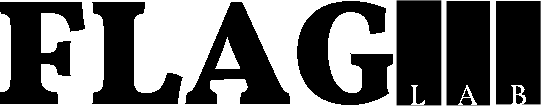
\includegraphics[width=0.7\textwidth]{Flag-logo.png}\\

                        \bigskip
                        \bigskip
                        \bigskip
                        \bigskip
                        \bigskip
                        \bigskip

                        
                        
\includegraphics[width=0.5\textwidth]{logo_uniandes.jpg}
                        %
                    \end{minipage}%
                    \begin{minipage}{0.55\textwidth}
                        \centering
                        Quantum-safe lattice-based abstractions in functional programs\\[1cm]
                        \fontsize{50}{60}
                        \selectfont
                        \textbf{Daniel Barrero${}^1$} \hspace{0.5cm} \textbf{Valérie Gauthier${}^1$} \hspace{0.5cm} \textbf{Nicolás Cardozo${}^1$}\\
                        \fontsize{40}{50}
                        \selectfont
                        ${}^1$Universidad de los Andes\\
                        \texttt{dr.barrero2562@uniandes.edu.co}
                    \end{minipage}%
                    \begin{minipage}{0.25\textwidth}
                    \centering
                        
\includegraphics[width=0.25\textwidth]{crypto_0.png}

                        \bigskip
                        \bigskip
                        
\includegraphics[width=0.6\textwidth]{pil-logo.png}
                        %
\includegraphics[width=0.5\textwidth]{logo_uniandes.jpg}
                    \end{minipage}
                    
                };
        \end{tikzpicture}
    \end{center}
    \vspace{2cm}
    \begin{multicols*}{3}
        \fontsize{49}{59}
        \selectfont
        \section{Quantum-safe Cryptography}\\
        
        Shor's quantum algorithm, published in 1994, demonstrated that factorization-based cryptography is no longer safe in the face of large-scale quantum computers.
        
        \[
    S_{i,j} =
        \begin{array}{ccccccc}
           \          & \      & |00\rangle & |01\rangle & |10\rangle & |11\rangle & \ \\
           |00\rangle & \vline & 1          & 0          & 0          & 0          & \vline\\
           |01\rangle & \vline & 0          & 1          & 0          & 0          & \vline\\
           |10\rangle & \vline & 0          & 0          & 1          & 0          & \vline\\
           |11\rangle & \vline & 0          & 0          & 0          & e^{i\theta_{k-j}}          & \vline
        \end{array}
\]


    %This begs the question of quantum-safe encryption protocols, for which \emph{the more, the better} rule applies.

    %For instance, the SIDH(KE) protocol was broken in 2022 by an efficient classical algorithm. ----> Have this to mention verbally, as I present the poster.


    % NIST standardization process, and its motivations.



    In 2015, the NSA announced its transition to quantum-resistant algorithms, in recognition of threats such as (1) \emph{Harvesting attacks:} store today's keys and cyphertexts to break later, (2) \emph{Forging signatures for old keys}, (3) \emph{Implementing new cryptography at scale takes a long time}.
    

    The following are the winners as of August 2024:
    
    \begin{itemize}
        \item CRYSTALS-kyber${}^*$
        \item CRYSTALS-dilithium${}^*$
        \item FALCON${}^*$
        \item SPHINCS+
    \end{itemize}

 
    \section{Lattice-based cryptography}\\
    
    Lattices offer the possibility of grounding cryptography on operations as simple as matrix multiplication and vector addition, where a lattice is a periodic grid in space (of any dimension), defined as the $\mathbb{Z}$-span of a basis for $\mathbb{R}^n$:
    
    \fontsize{45}{45}
    \selectfont
    \[
        L(B) = \{a_1\mathbf{b_1} +...+ a_n\mathbf{b_n} | a_i \in \mathbb{Z}, \mathbf{b_i} \in B\}.
    \]

    \begin{center}
        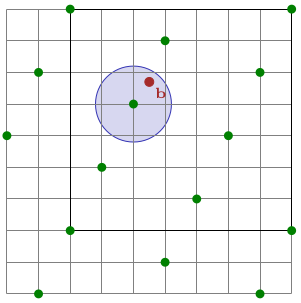
\includegraphics[width=0.22\textwidth]{lwe.png}
    \end{center}
    
    \fontsize{49}{58}
    \selectfont

    Computationally hard problems arise when the dimension of the lattice becomes large. In the relation
    
    % the most essential example being the \emph{shortest vector problem} (SVP, SVP${}_\gamma$).
    
    % In the related \emph{learning with errors} (LWE) problem, a public key cryptosystem is given by the relation

    \[
        \mathbf{b}^t = \mathbf{s}^t \mathbf{A} + \mathbf{e}^t,
    \]

    the public key is the random matrix $\mathbf{A}$ and the secret key is the vector $\mathbf{s}$. Recovering such key from the cyphertext $\mathbf{b}$ is as hard as solving the \emph{shortest vector problem} (SVP, SVP${}_\gamma$), which is known to be NP-hard.\\

    \section{Current Shortcomings}

    The best PQC algorithm so far is \emph{CRYSTALS-kyber}, which in a chat encryption scenario is known to

    \begin{itemize}
        \item Increase runtime by a factor of 2.3
        \item Increase energy consumption by 3.1
        \item Have 70 times more data overhead
    \end{itemize}

    These complications are due to internal hashing and \emph{discrete Fourier transforms} (DFTs), which occur iteratively in the encryption process.\\

    \section{Operad-based cryptography}
   
    \bigskip

     We may therefore attempt to simplify such sequences of operations. For this we will use the theory of \emph{operads}, whose objects represent \emph{operation composition}.

    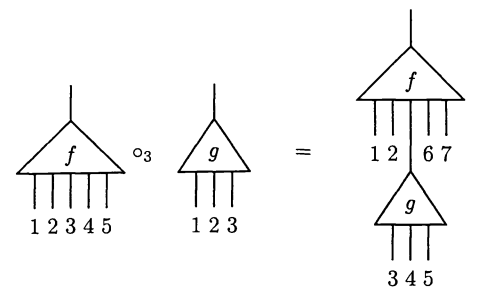
\includegraphics[width=0.29\textwidth]{fig1Intromss02.png}

    The fact that the best standards rely on property-preserving transformations (a.k.a. homomorphisms) to simplify computational complexity encourages this approach even further.

    % Maybe mention that modern crypto, such as CRYSTALS-Kyber, use module theory? (M_LWE)

    \section{A declarative language for quantum-safe cryptography} 

    \begin{itemize}
        \item The implementations of today's best protocols are written in languages such as C, which lack the expressiveness to express the operations naturally. This adds computational overhead and hides the intrinsic complexity of the scheme.
        \item Functional languages such as Haskell allow programmers to define category-theoretic abstractions in a way that is mathematically clear and natural. 
        
        \item[] 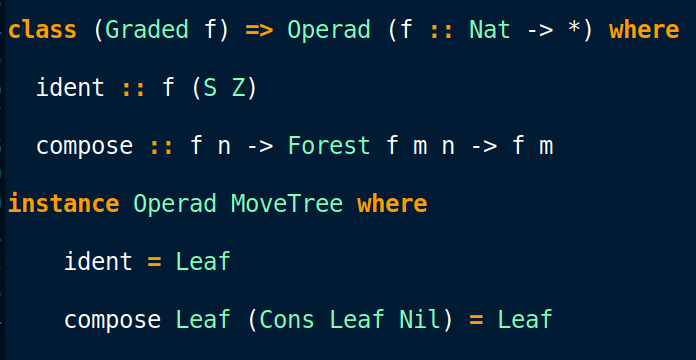
\includegraphics[width=0.29\textwidth]{toyOpds.png}
        
        \item In this project, we create the language SILVER, %Safely Implemented, Lattice-based Verifiable Encryption Resource.
     which will be \textbf{safe, expressive, and maintainable}. This will follow from the almost verbatim correspondence between mathematical definitions and type/typeclass declarations in our purely functional language (c.f. \emph{Curry-Howard correspondence}), together with the type-check requirement for the execution of a program.
    \end{itemize}
    
    
     % \flushright
     %     
\includegraphics[width=0.22\textwidth]{pil-logo.png}

     
    
    \end{multicols*}
        
\end{document}